\documentclass{utue} %utue.cls required for Uni Tuebingen corporate design
\usepackage{amsmath}
\usepackage{mathrsfs}
\usepackage[hidelinks]{hyperref}
\usepackage[all]{hypcap}
\def\sectionautorefname{Section}
% Values for title generation
\title{Cuda Implementation of Advanced Pencil Sketch Filter}
\author{Andreas Altergott, Raphael Braun, Stefan Burnicki}
\date{\today}

% Subtitle is optional. It represents what kind of work you did.
\subtitle{Practical course:\\Massive Parallel Programming SS2014}
\begin{document}

% You can place a teaser as follows. (Otherwise, just uncomment the following part)
\teaser{
    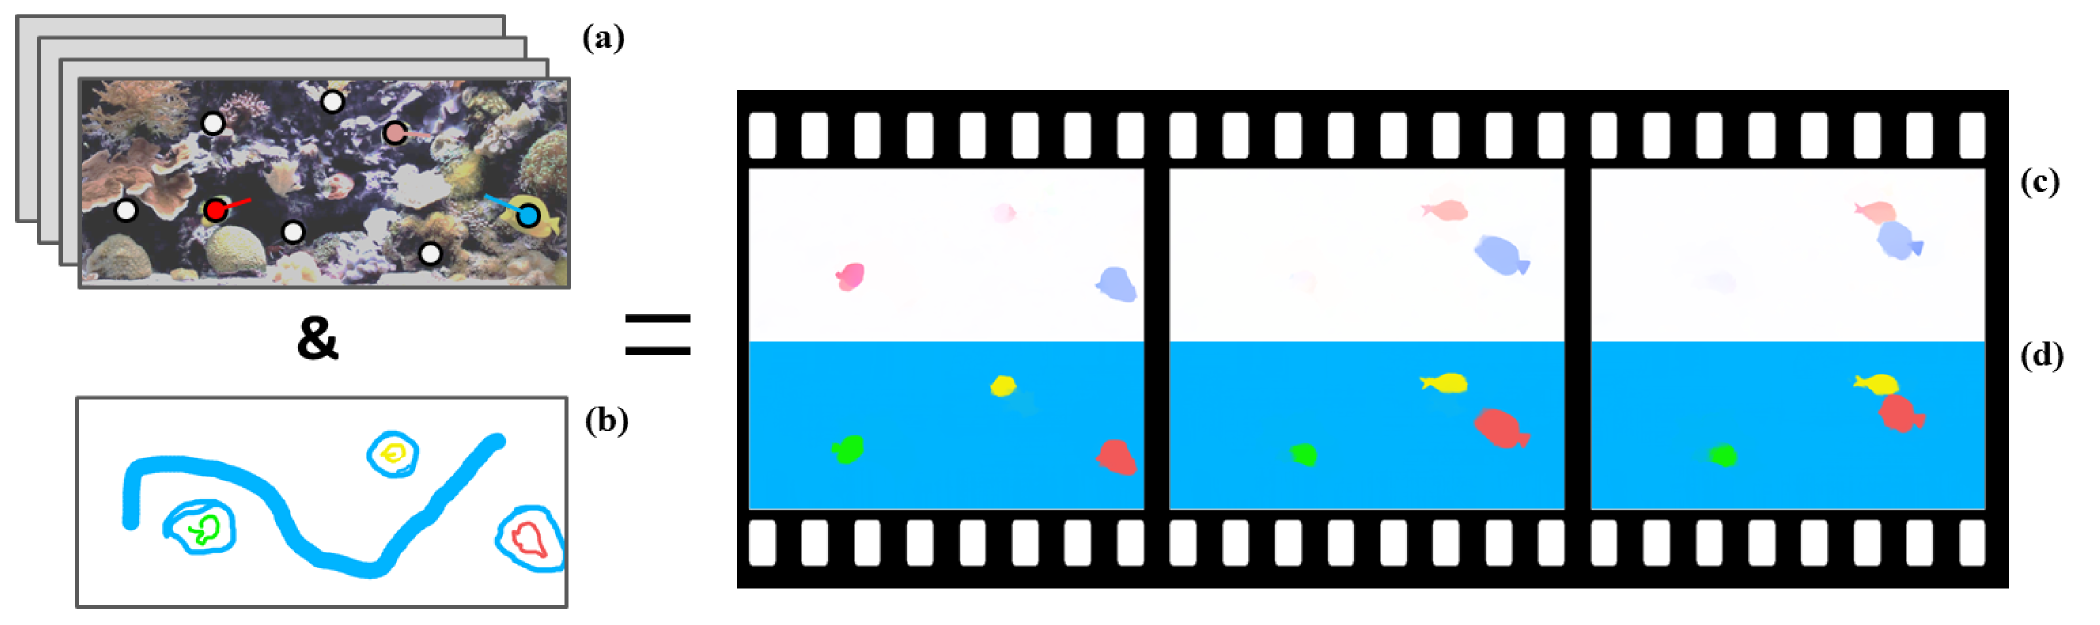
\includegraphics[width=.9\textwidth]{images/teaser.jpg}
    \caption{\label{fig:teaser} TODO}
}     

% Creates title of document and additional title page.
\maketitle 
 
\section*{Abstract} 
This paper describes the Cuda implementation of an advanced pencil sketch
filter, based on the work of Cewu Lu, Li Xu and Jiaya Jia\cite{mainPaper}.  It
explains the used methods of the original paper and discusses the derived
implementations for parallel computing. Details of the most complex
kernels are explained throughout the paper, as well as some important 
improvements to gain performance. The result of this work are extremely
fast computation times and very realistic pencil sketch images.



\section{Introduction}
Throughout time artist have perfected the art of creating pencil drawings in all
thinkable styles, ranging from completely abstract to stunningly photorealistic.
However, such skills are rare, and only well trained artists or passionate hobby
artists are able to actually create pleasing looking images using nothing but
the eye, a paper, and a pencil. Today, in a time where cameras can be used to
capture a real world scene in a matter of milliseconds, with accurate proportions and
colors, without requiring special skills, the need for pencil sketches seem to be gone.
After all, photographs do not convey the same emotions that sketches do. There is a certain
timeless flair to pencil sketches that makes them just nice to look at.

For this reason designing an image filter which produces a pencil sketch from
a regular photograph is an exciting task. The filter described in
\cite{mainPaper} is such a filter, which consists of two stages: sketching the
outlines and drawing the shading. In the sketch stage the filter calculates several
line convolutions and the shading stage solves a huge linear system of
equations. Both tasks are computationally rather expensive and according to the
authors their implementation of the filter takes 2 seconds to run on a
$600\times 600$ image. \autoref{fig:teaser} shows input, intermediate
results and the final result of the filter.

This report presents our efforts to implement the entire filter on the GPU using
Cuda to gain realtime results. The structure of the report is as follows: The
filter itself is described in \autoref{method}, then in
\autoref{gpu-implementation} we describe our implementation using Cuda.
\autoref{performance} shows our benchmark results for various input images
and in \autoref{future-work} some possible optimization and applications for our
implementation are pointed out.


\section{Previous Work}
This work is based on \cite{mainPaper}, as this paper describes the filter that
is implemented. The filter requires quite some parameters. In the original paper
they use a parameter learning approach to automatically select those parameters.
In this work the filter is kept slightly simpler than in the origin paper, e.g.
the line filter is slightly simplified and the filter parameters are left as
user controllable options. 

Another GPU-sketch-filter is described in \cite{Lu:2010:IPS}, though it uses the
a regular shaderpipeline. Based on the neighborhood informations of each pixel
it calculates weather to place a stroke at this point or not. The strokes are
then rendered as stroke-textures. The strokes are made in three different detail
layers based on the gradientmagnitude. Furthermore it is possible to filter
animations using optical flow. The greatest difference to the filter that we
implement is that they calculate each individual pencil or brush stroke based on
the gradient and then render those strokes using stroke-textures. Our method
uses traditional filters to alter the original image, which produces better
pencil sketches with respect to the tonal appearance. However their filter is
more versatile, as it allows different painting stiles and techniques by
changing the stroke-textures and weighting the detail layers.


A partially GPU based method is described in \cite{Benard:2012:ASC}. However
they concentrate on rendering temporal coherent line drawing animations from a
given 3D-scene. First they find active contours that are then adapted throughout
the animation. The result pictures are rendered by parameterizing the and then
add a certain style to the path. While this method yields amazing results for
very stylistic animations, it needs 3D input data.


\section{Method} \label{method}
The filter considers \textit{line scetching} and \textit{shading} separately.
The following subsections shed some light on how both stages work precisely.

The input for the filter is a regular RGB-image $I_{rgb}$. In the first step a
grayscale image $I_g$ is calculated using the $Y$-channel of the
$YUV$-transformed image $I_{yuv}$. $I_g$ now serves as input for the future
steps.

\subsection{Line Sketching}
One prominent task of the filter is to create sketchy looking outlines. The main
objective here is to mimic freehand sketching, which is typically done by
drawing short straight lines aligned to the outlines. The outlines are detected
using a simple gradient operator. Then each pixel is assigned to a line
direction and finally the pixel is drawn as part of its line.

\paragraph{Gradient Image}
The Outlines are detected and stored in the image $G$ using gradient magnitudes:
\begin{align*}
  G = ((\partial_x G)^2 + (\partial_y G)^2)^{\frac{1}{2}}
\end{align*}
In the center of \autoref{fig:sketch-steps} you can see how $G$ looks like.

\paragraph{Line Convolution Filter}
Given just the gradient magnitudes $G$ for each line direction $i \in
\lbrace 1,\cdots,N\rbrace$ where $N$ is the total number of lines, the convolution between
$G$ and each line segment $\mathscr{L}_i$ is calculated.
\begin{align}
  G_i = \mathscr{L}_i * G
  \label{eq:Gi}
\end{align}

The value $G_i(p)$ of pixel $p$ will be very big, if that pixel lies directly on
a line in $G$ (edge) and if $\mathscr{L}_i$ is following this line, such that only big
values are collected in the convolution. If the pixel doesn't lie on or close to
a line it can not gather high values and therefore stay dark. Pixels which lie
very close to edges can still gather some brightness if the
line segment $\mathscr{L}_i$ intersects the edge. This way lines in $G$ which
follow the direction of $\mathscr{L}_i$ show up and slightly overshoot in $G_i$.

Now to actually draw the lines, each pixel selects its maximum value from all
$G_i$:
\begin{align}
 L = \max(\lbrace G_i\rbrace) \quad \forall i \in  \lbrace1,\cdots,N\rbrace
 \label{eq:L}
\end{align}

In a final step $L$ is inverted, such that the lines are dark and the rest is
white. The result can be seen on the right side in \autoref{fig:sketch-steps}.

\begin{figure}[htb]
  \centering
  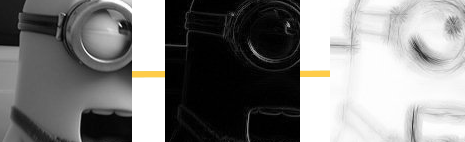
\includegraphics[width=0.4\textwidth]{images/sketch-steps.png}
  \caption{The intermediate results when calculating the line sketches. Left:
  input image, Center: Gradient image, Right: result $L$.}
  \label{fig:sketch-steps}
\end{figure}

\subsection{Shading}
The other important step in creating a believable pencil sketch image from a
natural image is to produce a hatching texture to create the shading. This is
done in two steps. First the histogram of the input image $I_g$ is matched to a
histogram model that was derived in \cite{mainPaper}. This way the tone
distribution is forced to correspond to tone distributions that were measured in
real pencil sketch images. Then the image of a given hatching pattern is used to
render the hatching texture for the input image. 

\paragraph{Histogram Matching}
Tones in natural images do not follow any specific pattern. In pencil drawings
however the tones are basically created only by two basic tones, namely the
white paper and the graphite strokes in different strengths. Heavy strokes are
used in very dark areas, mid tone strokes are used to produce impression of 3D
layered information and in bright areas the paper is just left white.
\autoref{fig:real-histograms} shows the tone distributions of some real pencil
sketches. One can easily see the three regions, the peak in the dark regions,
which represent the heavy strokes, the constant distribution in the mid tones,
which are used for the layering and very much bright pixels, originating from
the white paper, that was just left blank.

\begin{figure}[htb]
  \centering
  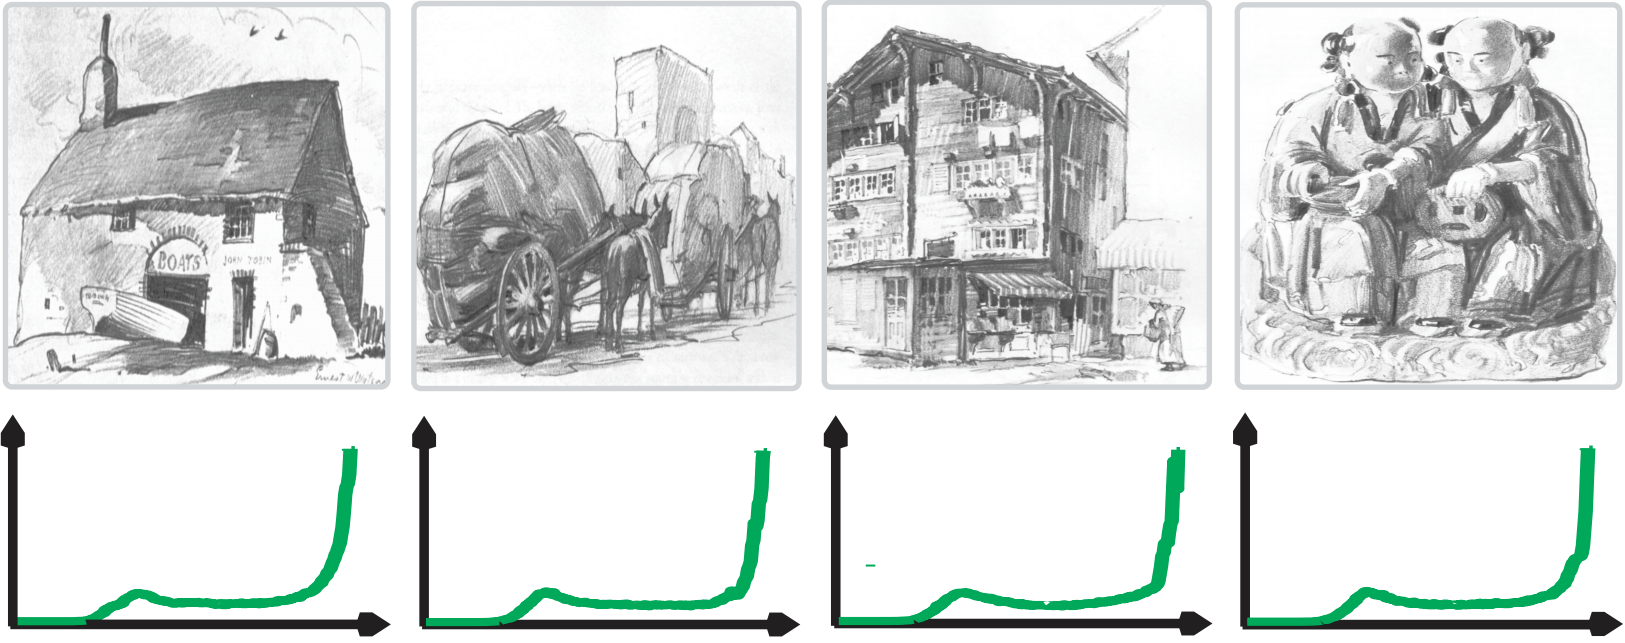
\includegraphics[width=0.4\textwidth]{images/real-histograms.png}
  \caption{Examples for real pencil sketches and their measured tone
    distributions. Note: This image was taken from \cite{mainPaper}}
  \label{fig:real-histograms}
\end{figure}

\cite{mainPaper} used this observation to create a parametric histogram model
for pencil drawings which consists of three functions, which represent those
three tone levels:

For the bright part of the histogram they use a Laplacian distribution with a
peak at the brightest value. This adds some variation in the bright areas, which
originate from slight illumination variances or the use of a eraser.

\begin{align}
  p_1(v) = \frac{255}{\sigma_b} e ^{-\frac{255-v}{\sigma_b}} \label{eq:p_1}
\end{align}

The parameter for this function is just $\sigma_b$, which controls the sharpness of
the function. This distribution can be seen on the very right of the histograms
in \autoref{fig:real-histograms}.

The mid layer is composed of strokes with different pressures and therefore in
different gray levels. So the distributions of those gray levels is equally
distributed as indicated in the histograms in \autoref{fig:real-histograms}. To
represent this part a constant function was chosen to use all those possible
gray levels.

\begin{align}
  p_2(v) = \begin{cases} \frac{1}{u_b - u_a} & \text{if } u_d < v \leq u_b\\
    0 & \text{otherwise}
  \end{cases} \label{eq:p_2}
\end{align}

The controlling parameters for this function are the range boundaries $u_d$
and $u_b$.

Finally the dark region which shows up as this bell shaped peak in the dark
regions in \autoref{fig:real-histograms} is represented as a Gauss-curve. The
position and shape of the dark regions depend on the maximum pressure an artist is using,
and the softness of the pencil that is used.

\begin{align}
  p_1(g) = \frac{1}{\sqrt{2\pi \sigma_d}} e^{-\frac{(v-\mu_d)^2}{2\sigma_d^2}} 
  \label{eq:p_3}
\end{align}

The width of the bell is controlled with the parameter $\sigma_d$ and the
position with $\mu_d$.

Plots for the three functions can be seen in \autoref{fig:p}.

\begin{figure}[htb]
  \centering
  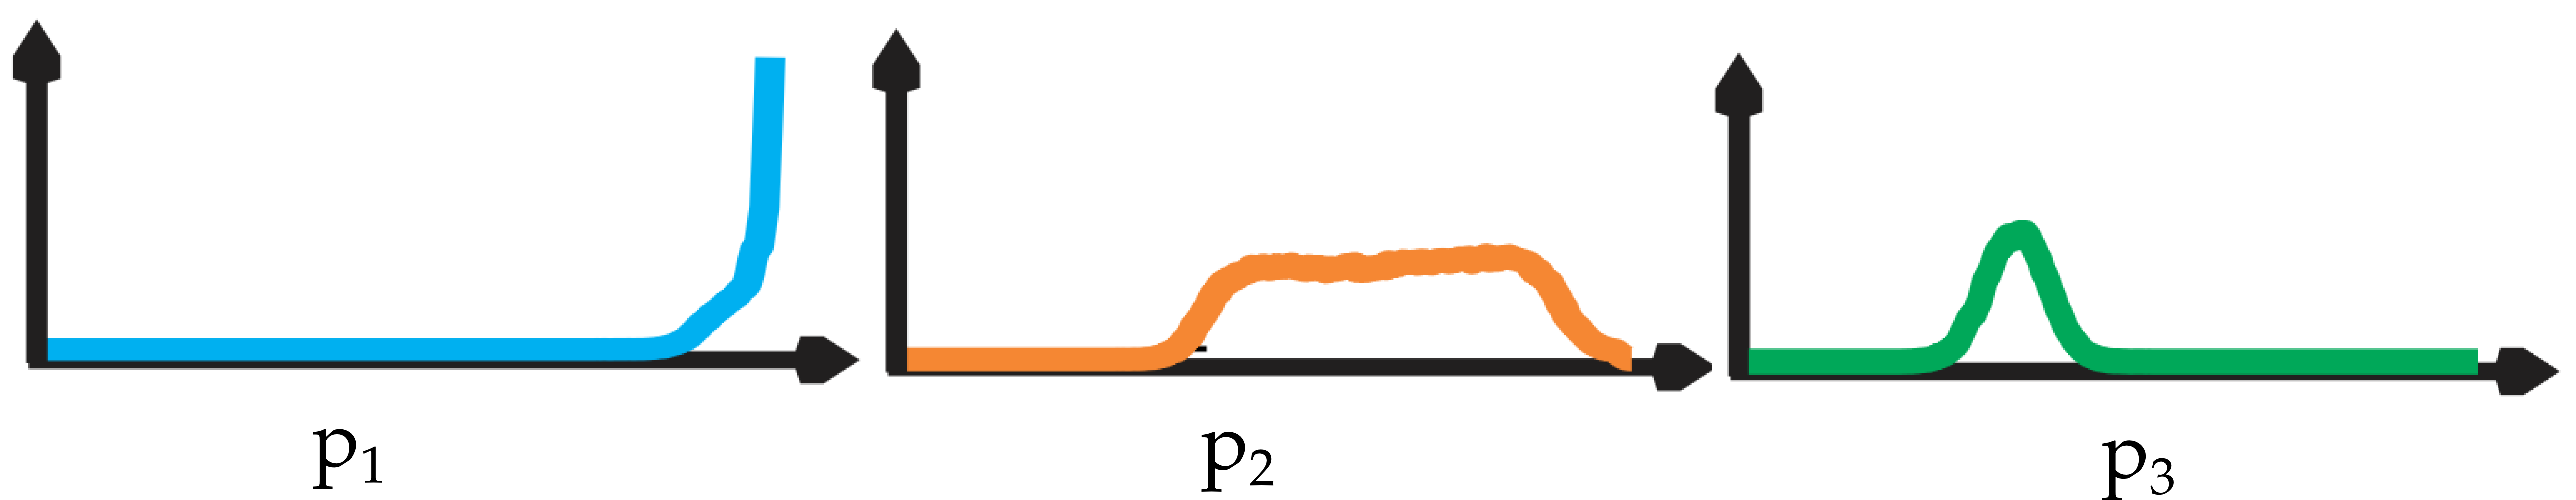
\includegraphics[width=0.4\textwidth]{images/p_i.png}
  \caption{Plots of the three functions $p_i$. Note: picture taken from
    \cite{mainPaper}.}
  \label{fig:p}
\end{figure}

The final tone distribution is now simply composited out of those three
function by creating a weighted sum from $p_1$, $p_2$ and $p_3$:
\begin{align}
  p(v) = \frac{1}{Z} \sum_{i=1}^{3}\omega_i p_i(v)
  \label{eq:p}
\end{align}
Where $Z$ is a normalization factor to make $\int_0^{255}p(v)dv = 1$ and the
$\omega_i$ are weighting parameters which can used to weight the importance of
the functions.

In \cite{mainPaper} they learned the parameters for those functions from a set
of different styled pencil sketches using Maximum Likelihood Estimation. We skipped this part and left those
parameters to be controlled by the user.

Histogram Matching is used to apply the tone distribution from \autoref{eq:p} to
the input image. The result $J$ is then used to calculate the hatching texture.
$J$ can be seen on the right side of \autoref{fig:hist-result}.

\begin{figure}[htb]
  \centering
  
\includegraphics[width=0.5\textwidth]{images/tone-result.png}
  \caption{Left input. Right: Result of Histogram matching for minions.}
  \label{fig:hist-result}
\end{figure}

\paragraph{Texturing}
The filter uses a men made pencil hatching pattern $H$. A human repetitively draws
at the same position to generate the correct tone in the hatching texture. A
exponential function can be used to simulate this process of placing multiple
strokes at the same position: $H(x)^{\beta(x)} \approx J(x)$. This corresponds
to drawing $H$ $\beta$ times at the same position to approximately match
the tone that is dictated by our tonal map $J$. In the logarithmic domain this
boils down to $\beta(x) \ln\left( H(x) \right) \approx \ln\left( J(x)
\right)$.

Just solving for $\beta$ in this equation is going to destroy the hatching
pattern because $\beta$ can be calculated for each pixel independently, such
that in the end $H^{\beta} = J$. Therefore a smoothness constraint is
introduced:
\begin{align}
  \beta = \arg \min_{\beta}\norm{\beta\ln(H) - \ln(J)}_2^2 + \lambda
  \norm{\nabla \beta}_2^2
  \label{eq:beta}
\end{align}
The smoothness weighting factor $\lambda$ can be used to determine how strong
the hatching pattern $H$ will show through in the result.

The hatching texture $T$ is then calculated as the pixelwise exponentiation
\begin{align*}
  T = H^{\beta}
\end{align*}
\autoref{fig:texture-result} shows the result for the minion.

\begin{figure}[htb]
  \centering
  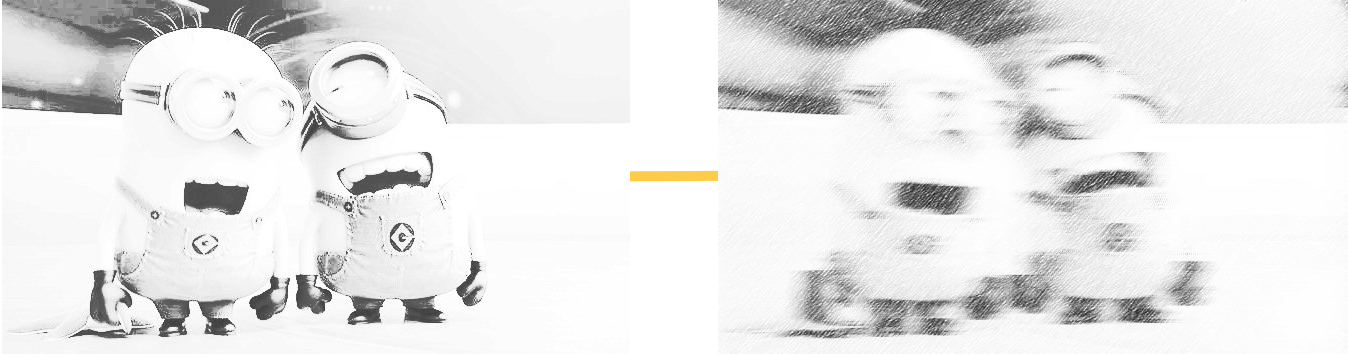
\includegraphics[width=0.5\textwidth]{images/texture-result.png}
  \caption{Left: $J$. Right: Result of texture rendering $T$.}
  \label{fig:texture-result}
\end{figure}



\paragraph{Combining Results}
Finally the results from the line sketching $L$ and the hatching texture $T$ is
combined to the finished pencil drawing $R$ by simply multiplying the images
pixelwise:
\begin{align*}
  R = L  \cdot T
\end{align*}

If desired it is also possible to create colored pencil drawings using the $YUV$
decomposed image $I_{yuv}$ from the beginning and replace the $Y$ channel with
$R$. The resulting RGB-image can then easily be calculated by a color space
transformation.

In \autoref{fig:final-result} both, grayscale and colored results are shown.

\begin{figure}[htb]
  \centering
  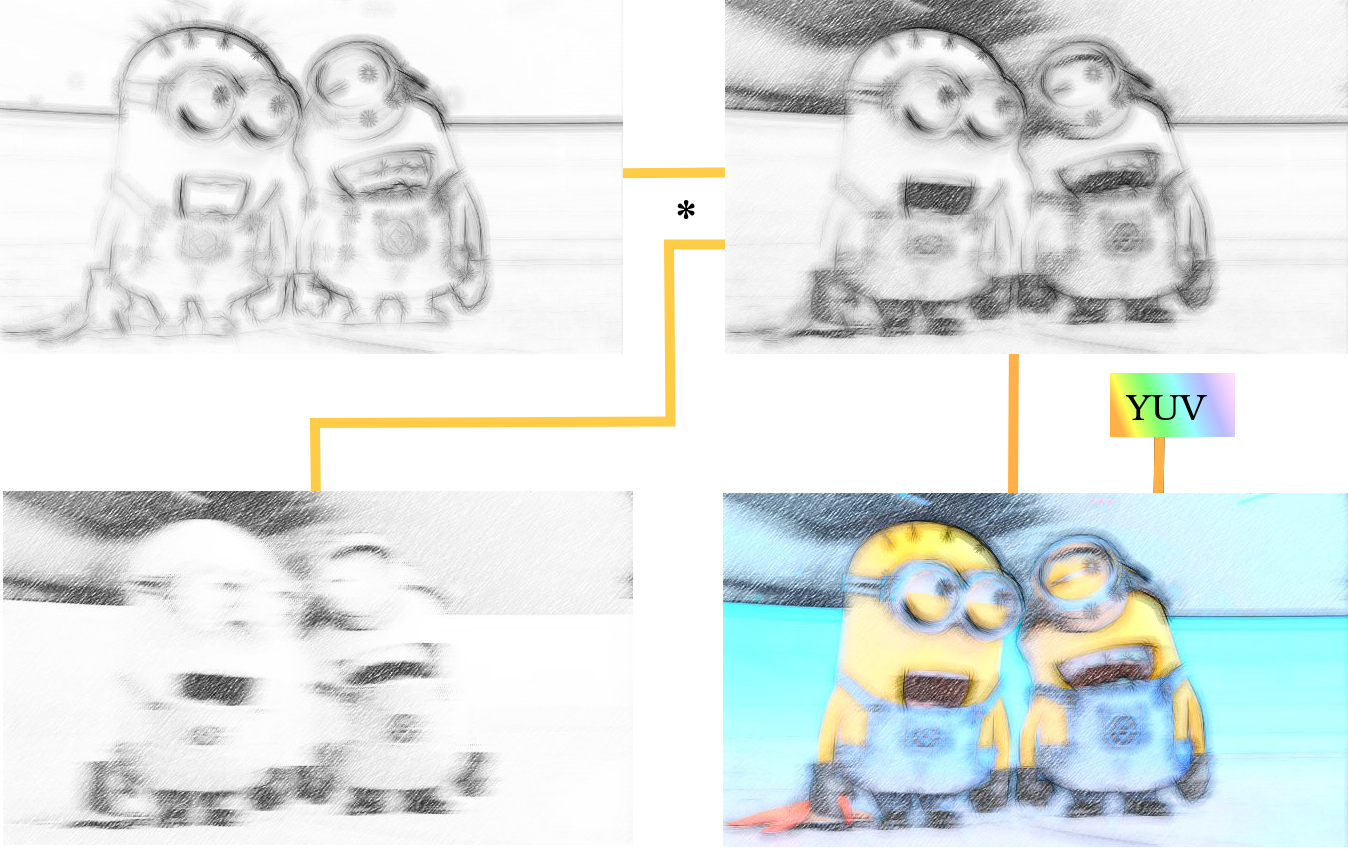
\includegraphics[width=0.5\textwidth]{images/final-result.png}
  \caption{combination of the results from the line drawing and shading.}
  \label{fig:final-result}
\end{figure}


\section{GPU Implementation} \label{gpu-implementation}

\begin{figure}[htb]
  \centering
  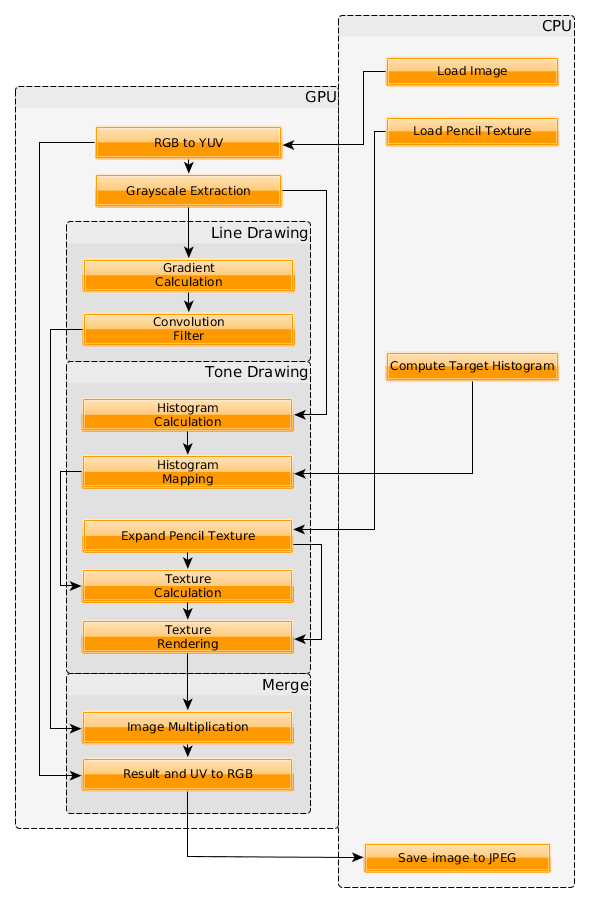
\includegraphics[width=0.5\textwidth]{images/pipeline.png}
  \caption{GPU and CPU pipeline of the implementation}
  \label{fig:pipeline}
\end{figure}

\autoref{fig:pipeline} displays the GPU and CPU pipeline of the implementation.
The first step loads the image, which happens on the CPU.  The conversion of
the image from RGB to YUV on the GPU is run in parallel with the loading of the
pencil textures on the CPU.  The next kernel extracts the gray-scale version of
the image from the RGB to YUV result.  The gray-scale version is used for the
gradient calculation, which is then applied to the convolution filter.  This
accomplishes the line drawing step.  In preparation for the tone drawing step,
the CPU is computing the target histogram.  The histogram calculation in the
tone drawing step receives the gray-scale version as the input image.  The
result is being passed to the histogram mapping, together with the computed
target histogram.  Another kernel receives the loaded pencil textures and
expands them to the image size.  The expanded textures and the histogram
mapping are being used for the texture calculation.  The last kernel in the
tone drawing, the texture rendering kernel, computes the result of the tone
drawing.  The last two kernels represent the merge.  One kernel combines the
results of the line drawing and the tone drawing step and generates the final
image.  The last kernel applies the coloring if requested and converts the YUV
back to RGB.  The CPU takes care of saving the image.

\subsection{Sketch Filter}
Calculating the grayscale image $I_g$ and Gradient $G$ on the GPU is no big
challenge. However the efficient implementation of the line convolution
calculation is more interesting.

To calculate the value $L(x)$, first all $G_i(x)$ have to
be computed (see \autoref{eq:Gi}) and the maximum from all line convolution
results is selected (see \autoref{eq:L}). The following paragraphs describe the
implementation of the Cuda-Kernel, which computes $L$ directly from $G$ given
the desired line length and strength.

\paragraph{Compute the line convolutions} 
To compute the convolution result $G_i(x)$ for pixel $x$ and line $i$ all values of $G$
along the line segment $\mathscr{L}_i$ are collected and averaged. The
convolution-kernel of the line segment $\mathscr{L}_i$ can be described as 
\begin{align*}
  k_i(p) = \begin{cases}
    \frac{1}{\text{line length} \cdot \text{line strength}} & p \text{ is part
    of } \mathscr{L}_i\\
    0 & \text{otherwise}
  \end{cases}
\end{align*}
Collecting the right pixels for the right line is done by iterating over the
pixels of a horizontal line with the desired length and strength. This line
starts at $x$. Then the coordinates are rotated to get the pixels for line $i$.
All line convolutions for one pixel is calculated by a single thread. The
results for a line is keep as maximum if it is bigger than all its predecessors. 

Finally the inversion, a gamma correction and clipping is used to create the
final value for $L(x)$:
\begin{align*}
  L(x) = \max(255 - \max(G_i)^{\gamma}, 50)
\end{align*}
The $\gamma$ parameter can be used to intensify or weaken the lines.

\paragraph{Shared Memory}
The same pixel values from $G$ have to be loaded from neighboring quite often.
Therefore it makes sens to use shared memory to speed up memory access.
As each pixel is calculated by a individual thread, and we can only use 1024
threads in one block we get blocks of size $32\times32$, as shown in
\autoref{fig:shared-memory}

\begin{figure}[htb]
  \centering
  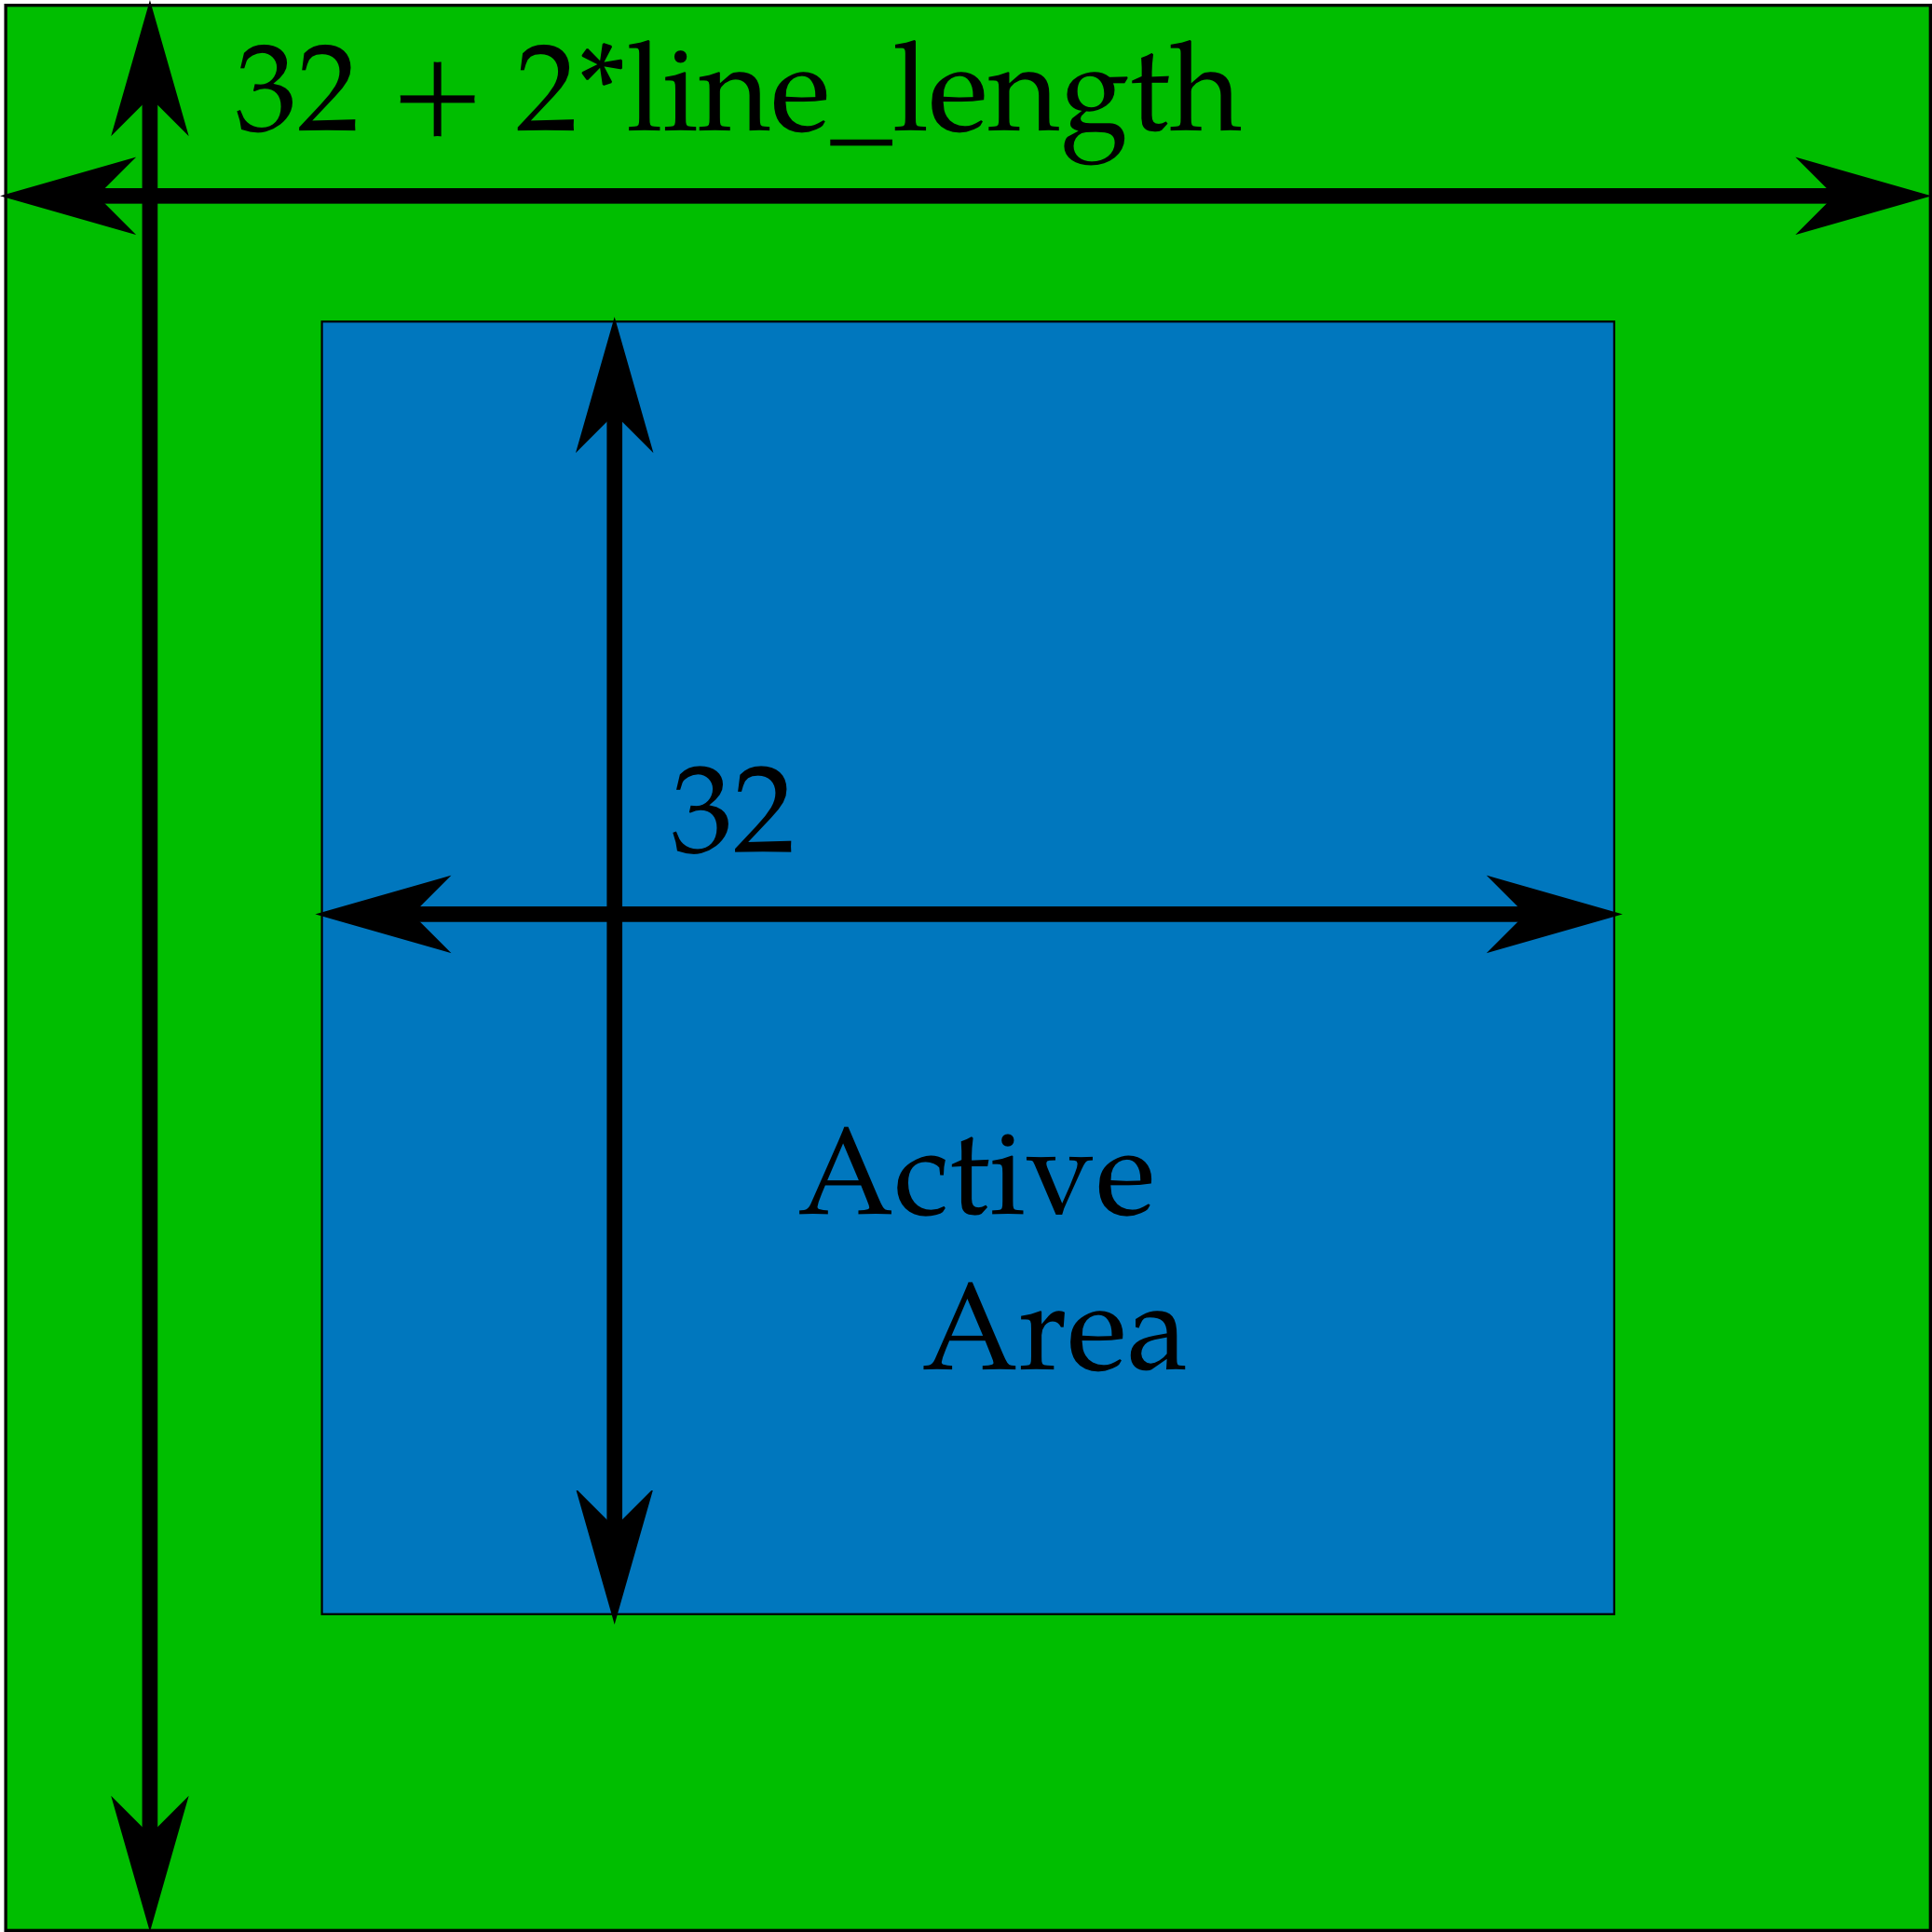
\includegraphics[width=0.2\textwidth]{images/shared-memory.png}
  \caption{Block and shared memory dimensions}
  \label{fig:shared-memory}
\end{figure}

On our device the maximum size of shared memory per block is $48kb$, so we can
only store a $109\times109$ block of float values. Therefore we only allow line
lengths up to 45 pixels.

The data from $G$ is copied by assigning the thread number to the linear
indexes of the data. As there is more data than threads, one thread copies
multiple data elements. The pattern is shown in \autoref{fig:shared-copy}.
\autoref{fig:shared-copy}.
\begin{figure}[htb]
  \centering
  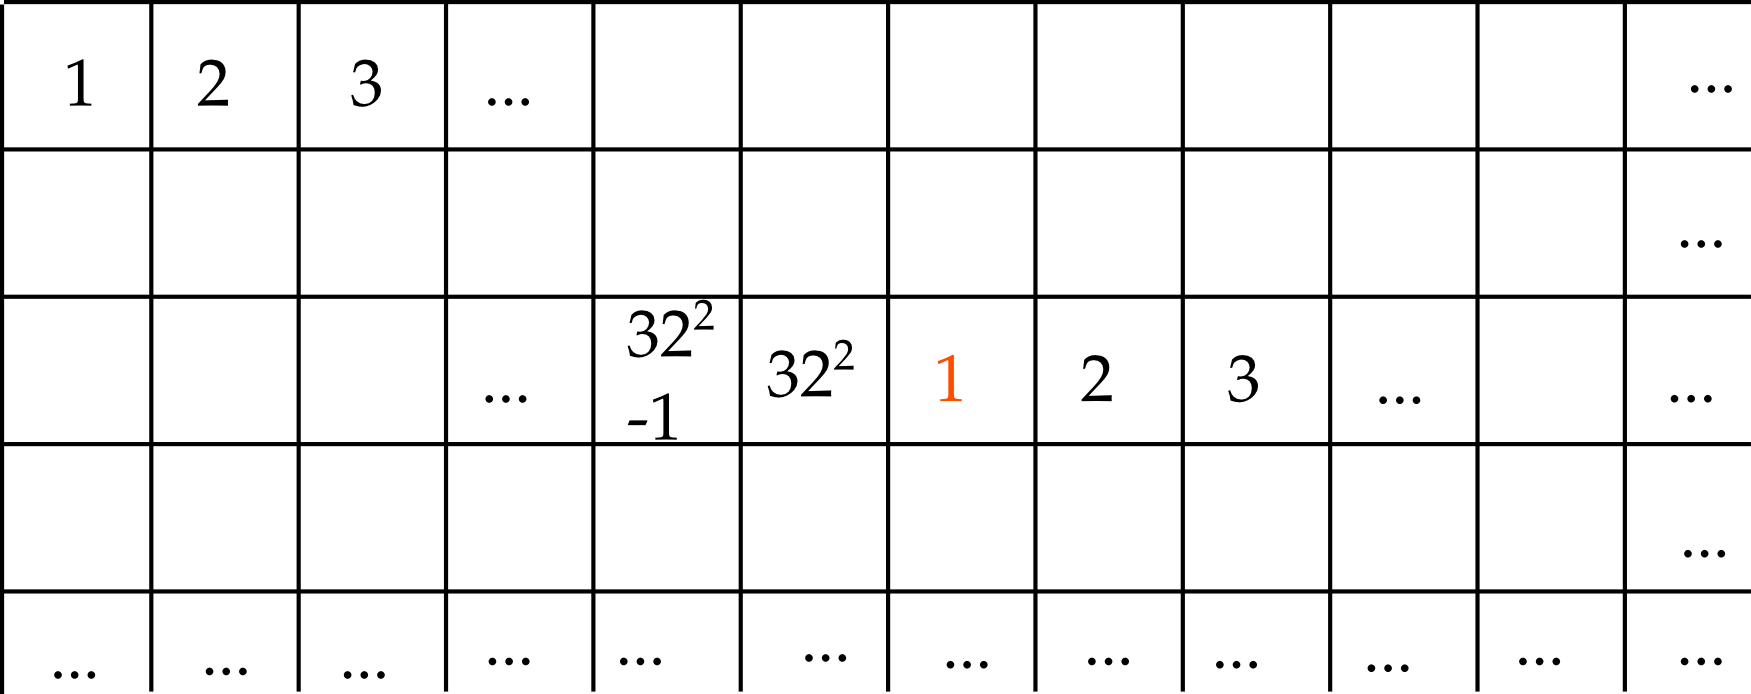
\includegraphics[width=0.5\textwidth]{images/shared-copy.png}
  \caption{Thread number assignment when copying the data from $G$ to shared memory.}
  \label{fig:shared-copy}
\end{figure}

The coordinate calculations for the line convolution computations are done such
that they generate the correct coordinates for the shared memory block. Due to
the coordinate rotations the access patterns are very chaotic, which might lead
to unavoidable bank conflicts.

Coordinates which lie outside the input image must not be included in the
copying process and later to calculate the convolution results.



\subsection{Histogram}
The histogram calculation uses the shared memory per block to compute a partial
histogram within each block.  Each block computes an additional accumulative
histogram with the use of parallel prefix sum.  The partial results are being
combined at the end of the kernel per thread, by accumulating the results in
global memory.  As we require a 256-bin histogram the shared memory per block
is only two times 256 Integers of size, one for the simple histogram and one
for the accumulative histogram.

\subsection{Histogram Matching}
The histogram matching is used to adjust the tone distribution of the 
grayscale image to match a specific target tone distribution by using
their corresponding histogram. In this context, the target tone
distribution is artificially created to be similar to those of pencil
sketches as explained above.

The cumulative target histogram is created on the CPU by simply applying
the the parametric model to the values 0 to 255 and summing it up with
the values below.
This step is done on the CPU as the target distribution only has to
be evaluated 256 times which is negligible effort and can be either be
precomputed or done while the GPU is busy with other steps of the pipeline.

Once this histogram is uploaded to the GPU it can be used together with
the histogram from the image created in the previous step to adjust the
tones of the grayscale image. This is done in a kernel with one thread
per image pixel. A thread will the obtain the tone value of the pixel
it corresponds to and look up it's cumulative probability value in
the source histogram map.
Afterwards, the cumulative target histogram is used in inverse to find
out which tone the value corresponds to in it. The pixel is then set to
the looked up target tone value.

The inverse lookup in the cumulative target histogram is implemented
as a binary search function which is used in the kernel. Although
one would think that a binary search is inefficient when multiple threads
are executed in a warp and search for different values, it really isn't.
As the cumulative target histogram map only consist of 256 values,
the binary search will need at maximum $log_2 256=8$ loop runs to end
up at the correct value. Because the threads are executed in a warp,
the branches might get executed in serial. However, there is just one 
real branching operation inside the loop body, which could double the
effort. Still, the total effort negligible in contrast to a linear search
through the map with a worst case complexity of 256.

\subsection{Texturing}
The \autoref{eq:beta} has the same shape as a Tikhonov regularization and
therefore can be solved exactly the same way by solving the following normal
equation:
\begin{align}
  \underbrace{(A A^T + \lambda \cdot \Gamma \Gamma^T)}_{A^*} x = \underbrace{A^T
  b}_{b^*}
  \label{eq:tikhonov}
\end{align}
$x$ is the solution image $\beta$ in vector shape. $A$ is a diagonal matrix.
Each diagonal element corresponds to one pixel in $\ln(H)$. $b$ is the
vectorized $\ln(J)$ image and $\Gamma$ is a diagonal matrix with two diagonals
which represents if multiplied to a vectorized image the gradient operator.

The iterative Conjugate Gradient solver from the cuda sparce library
(\texttt{cusp}) is used to solve the linear system $A^* x = b^*$.

For this the input images $\ln(J)$ and $\ln(H)$ are downloaded from the GPU,
feed into diagonal matrices from \texttt{cusp} then again uploaded to solve the
equation, once more downloaded and uploaded for the final composition with the
line image $L$.

Matrix $A*$ and vector $b^*$ (\autoref{eq:tikhonov}) could be calculated using
\texttt{cusp}. For this one would upload $\ln(H)$, $\ln(H)$ and $\Gamma$, and
use the matrix operations included in \texttt{cusp} to calculate the
matrix-matrix and matrix-vector multiplications. However it is much more
effective to construct $A^*$ and $b^*$ on the CPU and upload just those results,
because \texttt{cusp} needs an output target matrix for each operation. So a lot
of unnecessary memory needs to be allocated and used for the calculations on the
GPU.  Due to the nice structure of the matrices, $A^*$ and $b^*$  can be
calculated in $\mathcal{O}(n)$, with $n =$ number of pixel in the input image.
This is illustrated in \autoref{fig:matrix-mult}.

\begin{figure}[htb]
  \centering
  {\small
  \begin{align*}
    A*= \begin{pmatrix}
      a & 0 & -\lambda & 0 & 0 & 0 & 0 & \dots\\
      0 & b & 0 & -\lambda & 0 & 0 & 0 & \dots\\
      -\lambda & 0 & b & 0 & -\lambda & 0 & 0 & \dots\\
      0 & -\lambda & 0 & b & 0 & -\lambda & 0 & \dots\\
      0 & 0 & -\lambda & 0 & b & 0 & -\lambda & \ddots\\
      \vdots& &  &  &\ddots  \\
      0 & 0 & \dots & 0 & -\lambda & 0 & b & 0 & -\lambda\\
      0 & 0 & \dots & 0 & 0 &-\lambda & 0 & b & 0\\
      0 & 0 & \dots & 0 & 0 & 0 &-\lambda & 0 & a \\
    \end{pmatrix}
  \end{align*}
}
  \caption{Closed form for Matrix $A^*$. Substitute $a = \lambda +
  \ln(H(i))^2$ and substitute $b = 2\lambda + \ln(H(i))^2$ with $i$ being the line
in the matrix.}
  \label{fig:matrix-mult}
\end{figure}

According to our tests assembling the Matrix on the CPU gains a total speedup
of the program of factor 2.02 compared to the GPU method.


\section{Performance} \label{performance}
An important topic for the GPU implementation is of course the performance.
The described algorithm was implemented in a program that loads an image
from JPEG file, applies the filter to it, and saves it again to file.
Profiling this program showed that loading the image, allocating the
needed buffers, copying it to GPU, downloading it afterwards, and saving it
as JPEG to disk take the most time by far.

As these are factors that aren't under our control, we chose to measure
the time it takes to apply the implemented filter, and ignore the mentioned
overhead in our measurements. This approach is legitimate, as in time critic
applications the filter would be needed to be applied to multiple images. But this
would also mean that loading the image and copying it to GPU could be done while
the GPU is still busy with the previous image. Also the buffers can be reused,
such that their initialization doesn't count for performance measurements.

We measured the time the GPU pipeline needs to execute by repeating the
filter 100 times on the same image to compensate for fluctuation. We chose to do
our benchmarks with image resolutions known from common video formats:
DVD/PAL (720x576), 720p (1280x720) and FullHD (1920x1080). The filter
application to the DVD quality test image took 30 ms, the 720p version
took 60ms and the FullHD image took 130ms which are all a lot faster
then the original implementation \cite{mainPaper}.
Although the implementation is fast enough to be applied in real-time when watching
a video in DVD quality, it doesn't make sense to use it as a video filter.
The reason for this is that static textures are used for the shading effect
which would be repeated in each video frame, such that the shading would look
very unnatural.

To determine why our implementation takes so "long" for a FullHD image,
we profiled its application to the test image to find bottlenecks. We found out
that one step in the "hatch texture calculation" part takes nearly half the
time for the whole filter application. The crucial part is to upload matrix
$A^*$ to the GPU. If this \texttt{cusp} matrix could be directly created on the
GPU from the data that is already there, the performance of the filter would
roughly be doubled.  Unfortunately, we didn't find a good solution to this problem
in the scope of this project.


\section{Future Work} \label{future-work}
In the scope of our project we didn't jet implement the entire pipeline of the
original paper. 

The quality of our line sketch filter for example could be boosted by getting
rid of the blurriness, which would require one further processing step which is
described in \cite{mainPaper}.

As mentioned before, it would be nice if there was a way to construct matrix
$A^*$ and vector $b^*$ directly on the GPU with the data, that is already
there. This might be possible with the use of \texttt{cusp}s LinearOperator
classes.

Currently the parameters of the filter all have to be set manually. It would be
helpful to create some parameter presets, which can be selected and adapted on
the fly. Those presets could be created by the user on the fly and saved to disk
or learned from real pencil drawings as described in \cite{mainPaper}.

For this a GUI with realtime response would be great to immediately see the
response to parameter changes. 

If one could find a way to enforce temporal consistency in real time the filter
could be used to stylize entire video sequences. It might be worth it to take a
look at \cite{temporal-consistency} for this purpose. With precalculated optical
flow it might actually be possible to reach realtime performance.


\section{Conclusion}
Anyone


\bibliographystyle{alpha}
\bibliography{bibliography}


\end{document}

